% --------------------------------------------------------------------------- %
% Poster 
% --------------------------------------------------------------------------- %
%
% Poster template reference
% http://www.brian-amberg.de/uni/poster/
%
% --------------------------------------------------------------------------- %

\documentclass[a1paper,portrait]{baposter}
%\documentclass[a1paper,landscape]{baposter}
\usepackage{calc}
\usepackage{graphicx}
\usepackage{amsmath}
\usepackage{amssymb}
\usepackage{relsize}
\usepackage{multirow}
\usepackage{rotating}
\usepackage{bm}
\usepackage{url}
\usepackage{graphicx}
\usepackage{multicol}

\newcommand{\captionfont}{\footnotesize}

\graphicspath{{figures/}{../figures/}}
\usetikzlibrary{calc}

\newcommand{\SET}[1]  {\ensuremath{\mathcal{#1}}}
\newcommand{\MAT}[1]  {\ensuremath{\boldsymbol{#1}}}
\newcommand{\VEC}[1]  {\ensuremath{\boldsymbol{#1}}}
\newcommand{\Video}{\SET{V}}
\newcommand{\video}{\VEC{f}}
\newcommand{\track}{x}
\newcommand{\Track}{\SET T}
\newcommand{\LMs}{\SET L}
\newcommand{\lm}{l}
\newcommand{\PosE}{\SET P}
\newcommand{\posE}{\VEC p}
\newcommand{\negE}{\VEC n}
\newcommand{\NegE}{\SET N}
\newcommand{\Occluded}{\SET O}
\newcommand{\occluded}{o}

\usepackage{enumitem}% http://ctan.org/pkg/enumitem
\usepackage[utf8]{inputenc}
%Ionuţ-Alexandru Zaiţi, Ştefan-Gheorghe Pentiuc, Radu-Daniel Vatavu
%http://www.latex-community.org/forum/viewtopic.php?f=31&t=9084

%%%%%%%%%%%%%%%%%%%%%%%%%%%%%%%%%%%%%%%%%%%%%%%%%%%%%%%%%%%%%%%%%%%%%%%%%%%%%%%%
%%%% Some math symbols used in the text
%%%%%%%%%%%%%%%%%%%%%%%%%%%%%%%%%%%%%%%%%%%%%%%%%%%%%%%%%%%%%%%%%%%%%%%%%%%%%%%%

%%%%%%%%%%%%%%%%%%%%%%%%%%%%%%%%%%%%%%%%%%%%%%%%%%%%%%%%%%%%%%%%%%%%%%%%%%%%%%%%
% Multicol Settings
%%%%%%%%%%%%%%%%%%%%%%%%%%%%%%%%%%%%%%%%%%%%%%%%%%%%%%%%%%%%%%%%%%%%%%%%%%%%%%%%
\setlength{\columnsep}{1.5em}
\setlength{\columnseprule}{0mm}

%%%%%%%%%%%%%%%%%%%%%%%%%%%%%%%%%%%%%%%%%%%%%%%%%%%%%%%%%%%%%%%%%%%%%%%%%%%%%%%%
% Save space in lists. Use this after the opening of the list
%%%%%%%%%%%%%%%%%%%%%%%%%%%%%%%%%%%%%%%%%%%%%%%%%%%%%%%%%%%%%%%%%%%%%%%%%%%%%%%%
\newcommand{\compresslist}{%
\setlength{\itemsep}{1pt}%
\setlength{\parskip}{0pt}%
\setlength{\parsep}{0pt}%
}

%%%%%%%%%%%%%%%%%%%%%%%%%%%%%%%%%%%%%%%%%%%%%%%%%%%%%%%%%%%%%%%%%%%%%%%%%%%%%%
%%% Begin of Document
%%%%%%%%%%%%%%%%%%%%%%%%%%%%%%%%%%%%%%%%%%%%%%%%%%%%%%%%%%%%%%%%%%%%%%%%%%%%%%

\begin{document}

%%%%%%%%%%%%%%%%%%%%%%%%%%%%%%%%%%%%%%%%%%%%%%%%%%%%%%%%%%%%%%%%%%%%%%%%%%%%%%
%%% Here starts the poster
%%%---------------------------------------------------------------------------
%%% Format it to your taste with the options
%%%%%%%%%%%%%%%%%%%%%%%%%%%%%%%%%%%%%%%%%%%%%%%%%%%%%%%%%%%%%%%%%%%%%%%%%%%%%%
% Define some colors

% \definecolor{lightblue}{cmyk}{0.83,0.24,0,0.12}
\definecolor{lightblue}{rgb}{0.145,0.6666,1}

\definecolor{bgc_1}{RGB}{93, 194,232}
\definecolor{bgc_2}{RGB}{144, 190, 242}
\definecolor{hc_1}{RGB}{29,105,218}
\definecolor{hc_2}{RGB}{240,141,96}
\hyphenation{perform repetitions comfortable provides recognition triaxial}

%%
\begin{poster}%
  % Poster Options
  {
  % Show grid to help with alignment
  grid=false,
  % Column spacing
  colspacing=1em,
  % Color style
  bgColorOne=white,
  bgColorTwo=white,
  borderColor=lightblue,
  headerColorOne=black,
  headerColorTwo=lightblue,
  headerFontColor=white,
  boxColorOne=white,
  boxColorTwo=lightblue,
  % Format of textbox
  textborder=roundedleft,
  % Format of text header
  eyecatcher=true,
  headerborder=closed,
  headerheight=0.2\textheight,
  % textfont=\sc, An example of changing the text font
  headershape=roundedright,
  headershade=shadelr,
  headerfont=\Large \bf , %Sans Serif
  textfont={\setlength{\parindent}{0.2em}},
  boxshade=plain,
  % background=shade-tb,
  background=plain,
  linewidth=2pt
  }
%%% Eye Cacther %%%%%%%%%%%%%%%%%%%%%%%%%%%%%%%%%%%%%%%%%%%%%%%%%%%%%%%%%%%%%%%
{
	Eye Catcher, empty if option eyecatcher=false - unused
	% \includegraphics[height=3em]{conacyt_logo_v1.png}
}
%%% Title %%%%%%%%%%%%%%%%%%%%%%%%%%%%%%%%%%%%%%%%%%%%%%%%%%%%%%%%%%%%%%%%%%%%%
{\bf
  {
	open-corTeX: A 
	continuous integration framework for 
	open scientific communication
  }
}
%%% Authors %%%%%%%%%%%%%%%%%%%%%%%%%%%%%%%%%%%%%%%%%%%%%%%%%%%%%%%%%%%%%%%%%%%
{
	%\vspace{-0.3em} 
	{\smaller 
		Miguel Xochicale [miguel.xochicale@kcl.ac.uk] 
		} \\ 
	%\vspace{-0.5em}
	{\smaller
		School of Biomedical Engineering \& Imaging Sciences \\
		King's College London, UK 
	}
}
% % Logos
%   {% The makebox allows the title to flow into the logo, this is a hack because of the L shaped logo.
%   	\fbox{
%     \begin{minipage}{11em}
%     
%       \begin{center}
%       \includegraphics[height=2.95em]{uob_logo} \\
%       \end{center}
%       
%     \end{minipage}
%       }
%   } 


%%%%%%%%%%%%%%%%%%%%%%%%%%%%%%%%%%%%%%%%%%%%%%%%%%%%%%%%%%%%%%%%%%%%%%%%%%%%%%
%%% Now define the boxes that make up the poster
%%%---------------------------------------------------------------------------
%%% Each box has a name and can be placed absolutely or relatively.
%%% The only inconvenience is that you can only specify a relative position 
%%% towards an already declared box. So if you have a box attached to the 
%%% bottom, one to the top and a third one which should be in between, you 
%%% have to specify the top and bottom boxes before you specify the middle 
%%% box.
%%%%%%%%%%%%%%%%%%%%%%%%%%%%%%%%%%%%%%%%%%%%%%%%%%%%%%%%%%%%%%%%%%%%%%%%%%%%%%
    %
    % A coloured circle useful as a bullet with an adjustably strong filling
    \newcommand{\colouredcircle}{%
      \tikz{\useasboundingbox (-0.2em,-0.32em) rectangle(0.2em,0.32em); 
      \draw[draw=black,fill=lightblue,line width=0.03em] (0,0) circle(0.18em);}}
      


%%% Introduction %%%%%%%%%%%%%%%%%%%%%%%%%%%%%%%%%%%%%%%%%%%%%%%%%%%%%%%%%%%%%%%%%%%
\headerbox{Introduction}{name=intro,span=2,column=0,row=0}{
Full replication of scientific communication 
entails the release of code and data alongside with 
its documentation \cite{peng2011, heise2020, xochicale2019-github}.
However, there are various challenges, 
in the current system of open scientific communication, 
such as the evaluation of scientific work, 
speed in the communication process,
respect for the freedom of science and research,
dissemination and accessibility, digitization,
verifiability of scientific knowledge, quality, 
and prevention of misuse and scientific misconduct \cite{heise2020}.
That being said, the use of continuous integration tools 
\cite{luger-foreman-mackey-2019-github}
and containers \cite{xu2020-github}
is a starting point to tackle few of the previous challenges.
}


%%% open-corTeX %%%%%%%%%%%%%%%%%%%%%%%%%%%%%%%%%%%%%%%%%%%%%%%%%%%%%%%%%%%%%%%%%%%
\headerbox{open-corTeX}{name=opencortex,span=2,column=0,below=intro}{
open-corTeX is a prof-of-concept framework for open 
scientific communication and it is based on 
continuous integration (CI) of LaTeX documents by Luger and Foreman-Mackey 2019 \cite{luger-foreman-mackey-2019-github} 
and Github actions running docker images of full TeXlive, a.k.a containers, by Xu 2020 \cite{xu2020-github}.
Therefore, the open-corTeX framework involves two main steps: 
(a) the setting up of the yml file for the github action and 
(b) Github workflow. For the latter, user usually raises an issue, creates a branch, 
creates pull-request, asks for reviews and merges to master to then 
generate a full reproducible PDF document \cite{xochicale2020-opencortex}.

\vspace{-0.5em}
\begin{center}
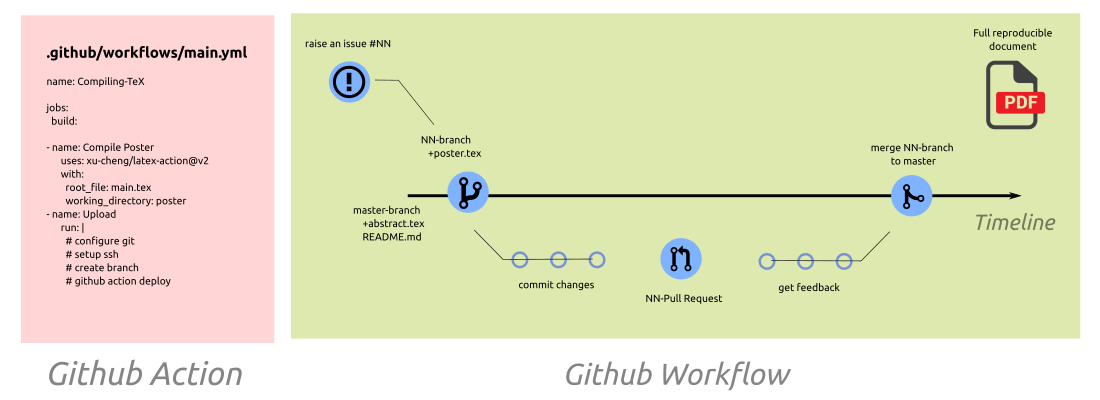
\includegraphics[width=1.0\textwidth]{open-cortex/versions/drawing-v00.png}  
\end{center}

}


  
%%% References %%%%%%%%%%%%%%%%%%%%%%%%%%%%%%%%%%%%%%%%%%%%%%%%%%%%%%%%%%%%%%%%%%%
\headerbox{References}{name=references,span=2,column=0,above=bottom}{
\tiny
\vspace{-0.4em} % Save some space at the beginning
\bibliographystyle{ieee}
\renewcommand{\section}[2]{\vskip 0.05em}

\begin{thebibliography}{1}
\itemsep=-0.01em
\setlength{\baselineskip}{0.4em}

\bibitem{peng2011}
Peng Roger D.
\newblock Reproducible Research in Computational Science.
\newblock In {\em Science} 334.6060 (2011),  doi: 10.1126/science.1213847

\bibitem{heise2020}
Heise Christian and Pearce Joshua M. 
\newblock From Open Access to Open Science: The Path From Scientific Reality to Open Scientific Communication.
\newblock In {\em  SAGE Open} 10.2 (2020), doi: 10.1177/2158244020915900 

\bibitem{xochicale2019-github}
Xochicale Miguel. 
\newblock Github repository for PhD thesis. 
\newblock Sep. 2019. doi: 10.5281/zenodo.3384281

\bibitem{luger-foreman-mackey-2019-github}
Luger Rodrigo and Foreman-Mackey Daniel.
\newblock Continuously-integrated Open-source Reproducible TeX.
\newblock https://github.com/rodluger/cortex.

\bibitem{xu2020-github}
Xu Cheng.
\newblock GitHub Action to compile LaTeX documents.
\newblock May 2020. https://github.com/xu-cheng/latex-action.

\bibitem{xochicale2020-opencortex}
Xochicale Miguel.
\newblock open-corTeX: A framework for open-accessible continuous integration for scientific communication
\newblock Github repository. Sep. 2020. https://github.com/mxochicale/rrts2020.

\end{thebibliography}
}


%%% Results %%%%%%%%%%%%%%%%%%%%%%%%%%%%%%%%%%%%%%%%%%%%%%%%%%%%%%%%%%%%%%%%%%%
\headerbox{Results}{name=results,span=1,column=2,row=0,aligned=intro}{
\LaTeX-document outputs for article, thesis, CV, poster and slides with the use of
 open-corTeX \cite{xochicale2020-opencortex}.

\vspace{-0.9em}
\begin{center}
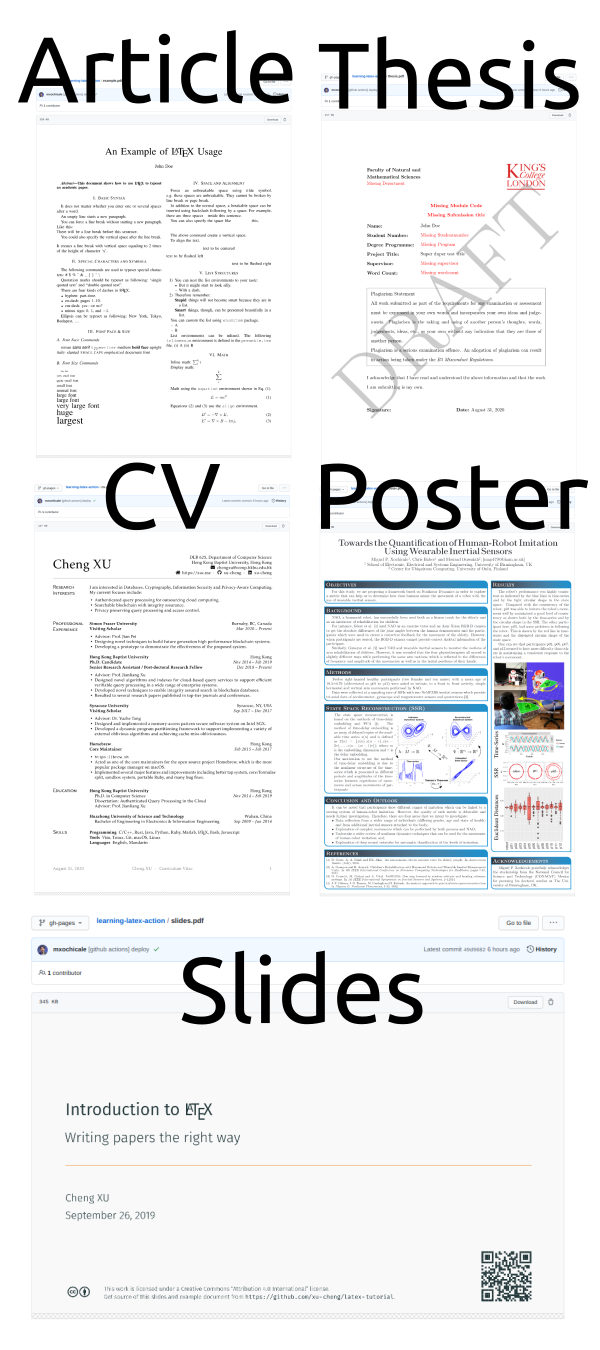
\includegraphics[width=0.9\linewidth]{results/versions/drawing-v00.png} 
\end{center}
}

\headerbox{Takeaways}{name=takeaways,span=1,column=2,below=results, above=bottom}{

$\bullet$
Tools such as CI and containers can improve reproduciblity 
because of their portability and lightweight
to produce the same output 
without regard to the operational system.
  
$\bullet$ The adoption of open-corTeX might led to scientific outcomes 
that are aligned to the principles of 
reproducibility, inclusiveness, transparency,
reusability and open accessibility. 

}


\end{poster}

\end{document}
